%%%%%%%%%%%%%%%%%%%%%%%%% NOTE %%%%%%%%%%%%%%%%%%%%%%%%%%%%
%% You can ignore everything from here until             %%
%% "Question 1: Introduction"                            %%
%%%%%%%%%%%%%%%%%%%%%%%%%%%%%%%%%%%%%%%%%%%%%%%%%%%%%%%%%%%
\documentclass[8pt]{article}
\usepackage{amsmath, amsfonts, amsthm, amssymb}  % Some math symbols
% \usepackage{fullpage}
\usepackage[a4paper, left=0.5in, right=0.5in, top=0.5in, bottom=0.5in]{geometry}
\usepackage{graphicx}
\usepackage[x11names, rgb]{xcolor}
\usepackage{graphicx}
\usepackage{tikz}
\usepackage{tcolorbox}
\usetikzlibrary{decorations,arrows,shapes}
\usepackage{float} % Add this package to control float placement
\usepackage{etoolbox}
\usepackage{enumerate}
\usepackage{listings}
\usepackage{algorithm}
\usepackage{algorithmic}
\usepackage{algpseudocode}
\lstset{
    language=Python,           % Set the language of the code
    basicstyle=\footnotesize\ttfamily,
    keywordstyle=\color{blue}, % Set color for keywords
    commentstyle=\color{gray}, % Set color for comments
    stringstyle=\color{red},   % Set color for strings
    numbers=left,              % Display line numbers on the left
    numberstyle=\tiny\color{gray}, % Style for line numbers
    frame=single,              % Add a frame around the code
    breaklines=true            % Allow line breaking
}


\setlength{\parindent}{0pt}
\setlength{\parskip}{5pt plus 1pt}

\newcommand{\N}{\mathbb N}
\newcommand{\E}{\mathbb E}
\newcommand{\V}{Var}
\renewcommand{\P}{\mathbb P}
\newcommand{\f}{\frac}


\newcommand{\nopagenumbers}{
    \pagestyle{empty}
}

\def\indented#1{\list{}{}\item[]}
\let\indented=\endlist

\providetoggle{questionnumbers}
\settoggle{questionnumbers}{true}
\newcommand{\noquestionnumbers}{
    \settoggle{questionnumbers}{false}
}

\newcounter{questionCounter}
\newenvironment{question}[2][\arabic{questionCounter}]{%
    \addtocounter{questionCounter}{1}%
    \setcounter{partCounter}{0}%
    \vspace{.25in} \hrule \vspace{0.4em}%
        \noindent{\bf \iftoggle{questionnumbers}{#1: }{}#2}%
    \vspace{0.8em} \hrule \vspace{.10in}%
}{$ $\newpage}

\newcounter{partCounter}[questionCounter]
\renewenvironment{part}[1][\alph{partCounter}]{%
    \addtocounter{partCounter}{1}%
    \vspace{.10in}%
    \begin{indented}%
       {\bf (#1)} %
}{\end{indented}}

\def\show#1{\ifdefempty{#1}{}{#1\\}}

\newcommand{\header}{%
\begin{center}
    {\Large \show\myhwname}
    \show\myname
    \show\myemail
    \show\mysection
    \show\hwname
\end{center}}

\usepackage{hyperref} % for hyperlinks
\hypersetup{
    colorlinks=true,
    linkcolor=blue,
    filecolor=magenta,      
    urlcolor=blue,
}

%%%%%%%%%%%%%%%%% Identifying Information %%%%%%%%%%%%%%%%%
%% For 312, we'd rather you DIDN'T tell us who you are   %%
%% in your homework so that we're not biased when        %%
%% So, even if you fill this information in, it will not %%
%% show up in the document unless you uncomment \header  %%
%% below                                                 %%
%%%%%%%%%%%%%%%%%%%%%%%%%%%%%%%%%%%%%%%%%%%%%%%%%%%%%%%%%%%
\newcommand{\myhwname}{DS221: Introduction to Scalable Systems}
\newcommand{\myname}{Naman Pesricha }
\newcommand{\myemail}{namanp@iisc.ac.in}
\newcommand{\hwname}{\textbf{Parallel Programming}}
\newcommand{\mysection}{SR - 24115}
%%%%%%%%%%%%%%%%%%%%%%%%%%%%%%%%%%%%%%%%%%%%%%%%%%%%%%%%%%%

%%%%%%%%%%%%%%%%%%% Document Options %%%%%%%%%%%%%%%%%%%%%%
\noquestionnumbers
\nopagenumbers
%%%%%%%%%%%%%%%%%%%%%%%%%%%%%%%%%%%%%%%%%%%%%%%%%%%%%%%%%%%

\begin{document}
\header

\begin{question}{Q1 \underline{OpenMP Prefix Sum (7.5 points)}

Prefix sum of a set of elements contained in an integer array, A, produces an integer array, B, such that
B[j] = sum (from i=0 to i=j) A[i]
Example, if A[] = \{5, 7, 3, 8, 2\}, B will be B[] = \{5, 12, 15, 23, 25\}

Write a OpenMP parallel program for parallelizing the above prefix problem. Input array A and output array B will be shared by the OpenMP threads. Different threads will deal with different disjoint elements of B. 

Experiment with array sizes of 10000, 20000 and 30000 integer elements. For each array, run your code with 2, 4, 8, 16, 32 and 64 threads. For a given array and given number of threads, run your code 5 times and obtain the average time across these 5 runs. Obtain speedups with respect to sequential execution. Write a report describing the methodology, experiments, results and observations. For results, give execution times, speedups as both numbers and grassph plots.
}


\begin{tcolorbox} [width = \textwidth]
\section*{1 Methodology}
\end{tcolorbox}

    The implementation of \texttt{prefixSumOMP} computes the prefix sum of an input vector \( A \) and stores the result in vector \( B \) using multiple threads with OpenMP. The approach divides the input array \( A \) into subarrays for each thread, calculates local prefix sums, and then adjusts these with offsets derived from the global prefix sums of previous threads. Below is the step-by-step methodology:

\begin{enumerate}
    \item \textbf{Input Partitioning:} \\
    The input vector \( A \) of size \( n \) is divided into \( t \) equal parts (for \( t \) threads). Each thread \( t_i \) is responsible for calculating the prefix sum of its assigned subarray \( A_i \). Let:
    \begin{itemize}
        \item \( A_0, A_1, A_2, A_3 \) be the subarrays handled by threads \( t_0, t_1, t_2, t_3 \), respectively.
    \end{itemize}

    \item \textbf{Local Prefix Sum Calculation:} \\
    Each thread calculates the prefix sum of its assigned subarray:
    \begin{itemize}
        \item Thread \( t_i \) starts at index \( \text{start} = i \times \frac{n}{t} \) and ends at \( \text{end} = (i+1) \times \frac{n}{t} \).
        \item The first element of \( B_i \) is set as \( B[\text{start}] = A[\text{start}] \).
        \item For subsequent elements:
        \[
        B[j] = A[j] + B[j - 1], \quad \forall j \in [\text{start} + 1, \text{end}).
        \]
    \end{itemize}

    Example:
    \begin{itemize}
        \item \( t_0 \) computes the local prefix sum for \( A_0 \) and stores it in \( B_0 \).
        \item Similarly, \( t_1, t_2, t_3 \) compute local prefix sums for \( A_1, A_2, A_3 \), respectively.
    \end{itemize}

    \item \textbf{Compute Offsets:} \\
    After completing local prefix sums:
    \begin{itemize}
        \item Each thread calculates the total sum of its subarray:
        \[
        \text{offsets}[i] = B[\text{end} - 1], \quad \text{for thread } t_i.
        \]
        \item Thread \( t_0 \) sets its offset to 0:
        \[
        \text{offsets}[0] = 0.
        \]
    \end{itemize}

    \item \textbf{Global Offset Adjustment:} \\
    Using the offsets:
    \begin{itemize}
        \item Thread \( t_0 \) requires no adjustment since \( \text{offsets}[0] = 0 \).
        \item Thread \( t_1 \) adds the sum of \( A_0 \) to all elements of \( B_1 \).
        \item Thread \( t_2 \) adds the cumulative sum of \( A_0 \) and \( A_1 \) to all elements of \( B_2 \), and so on.
    \end{itemize}
    
    Offsets are computed globally using a single-thread operation:
    \[
    \text{offsets}[i] = \text{offsets}[i] + \text{offsets}[i - 1], \quad \forall i > 0.
    \]

    \item \textbf{Adjust Local Prefix Sums (SIMD):} \\
    Each thread adjusts its local prefix sum using its respective offset:
    \begin{itemize}
        \item \( B[j] = B[j] + \text{offsets}[i], \quad \forall j \in [\text{start}, \text{end}). \)
    \end{itemize}
\end{enumerate}


\begin{figure}[H]
    \centering
    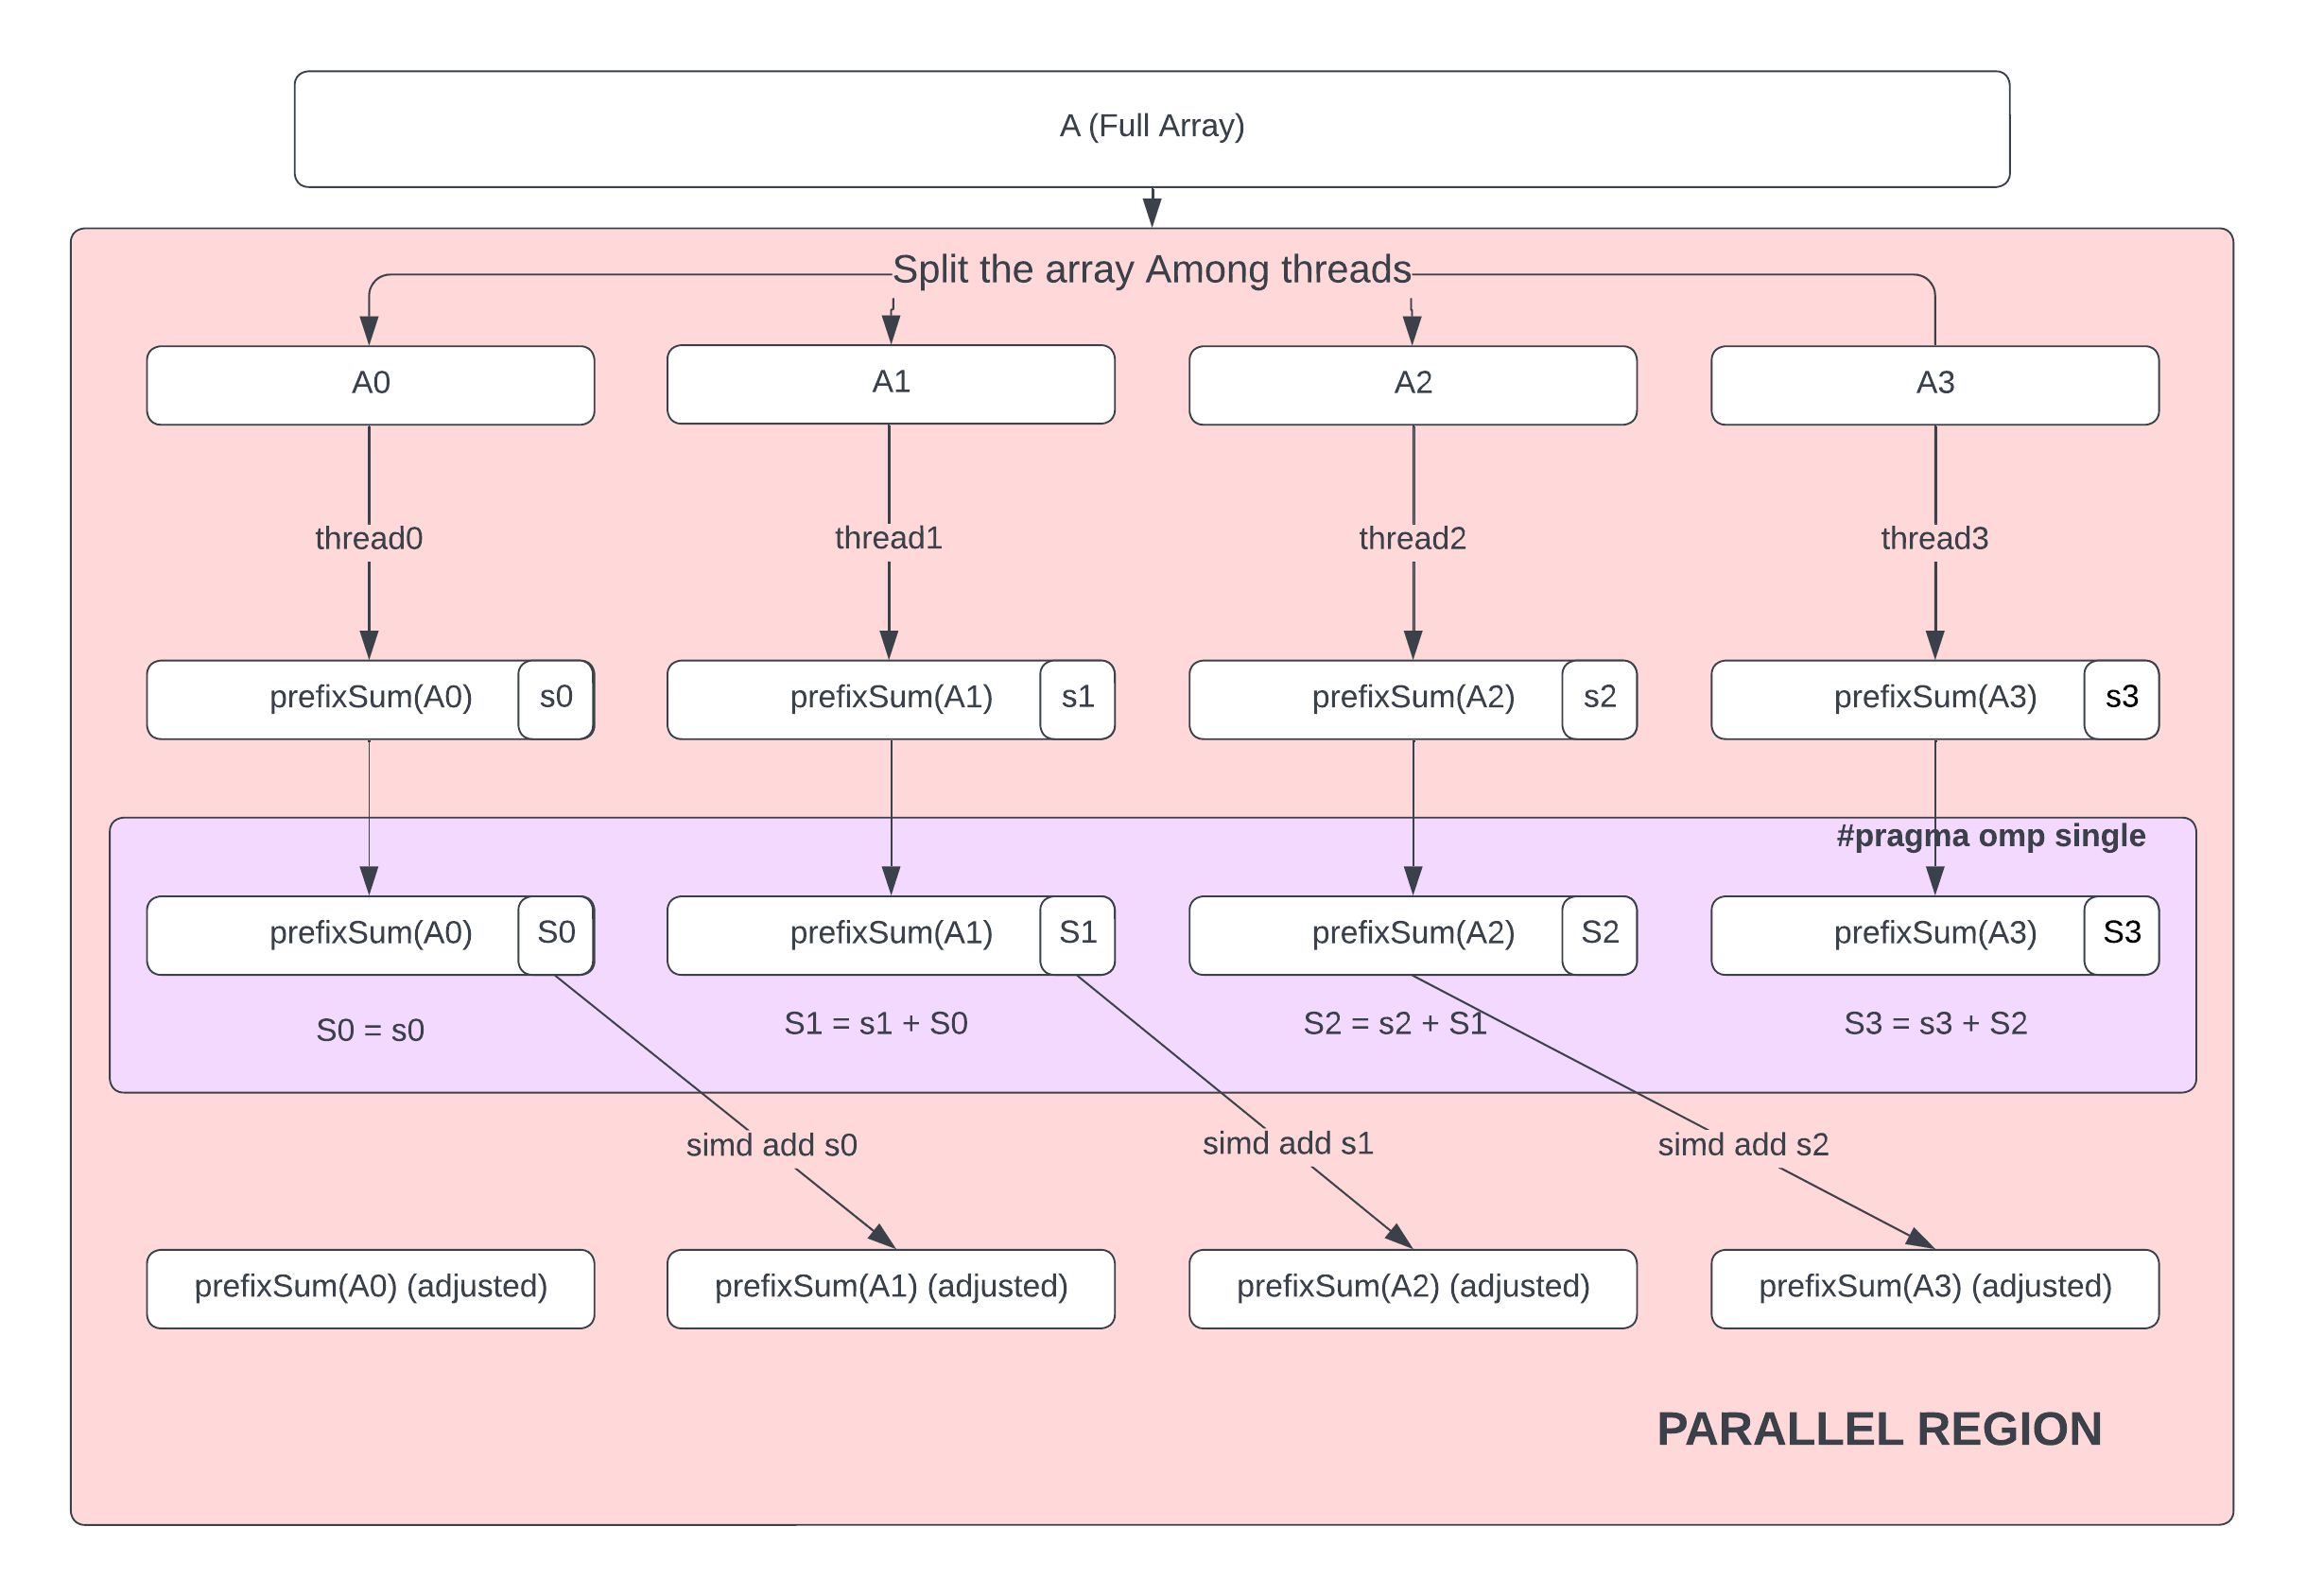
\includegraphics[width=0.9\textwidth]{images/openmp.png} % Adjust the width as needed
    \caption{Methodology for parallel prefix sum.}
    \label{fig:your_label}
\end{figure}

\underline{\textbf{\large{1.1 Example with 4 thread:} }}

\textbf{Input Array \( A \) (size 16):}
\[
A = [1, 2, 3, 4, 5, 6, 7, 8, 9, 10, 11, 12, 13, 14, 15, 16]
\]

\textbf{Step 1}: Partition \( A \) into Subarrays:
\begin{center}
            \item \( A_0 = [1, 2, 3, 4] \) for \( t_0 \)
            \item \( A_1 = [5, 6, 7, 8] \) for \( t_1 \)
            \item \( A_2 = [9, 10, 11, 12] \) for \( t_2 \)
            \item \( A_3 = [13, 14, 15, 16] \) for \( t_3 \)
\end{center}

\textbf{Step 2}: Local Prefix Sums
\begin{center}
    \item \( B_0 = [1, 3, 6, 10] \)
    \item \( B_1 = [5, 11, 18, 26] \)
    \item \( B_2 = [9, 19, 30, 42] \)
    \item \( B_3 = [13, 27, 42, 58] \)
\end{center}


\textbf{Step 3}: Calculate Offsets
\[
\text{offsets} = [0,10,26,42].
\]

\textbf{Step 4}: Global Offset Adjustment
\[
\text{offsets} = [0,10,36,78].
\]

\textbf{Step 5: Adjust Local Prefix Sums}
\begin{center}
    \item Adjust \( B_1 \): \( [15, 21, 28, 36] \)
    \item Adjust \( B_2 \): \( [45, 55, 66, 78] \)
    \item Adjust \( B_3 \): \( [91, 105, 120, 136] \)
\end{center}


\textbf{Final Result \( B \):}
\begin{tcolorbox} 
{\[
B=[1,3,6,10,15,21,28,36,45,55,66,78,91,105,120,136].
\]}
\end{tcolorbox}

\underline{\textbf{\large{1.2 Time Complexity}}}

The time complexity for the program is: 

\begin{large}
    \[
    T(n,t) = O\left(\frac{2n}{t} + t\right) + parallelization\ overheads
    \]
\end{large}
\begin{center}
    \item Step 1 and 2 : O(n/t).
    \item Step 3 and 4 : O(t).
    \item Step 5 : O(n/t)    
\end{center}


\hrule
\begin{tcolorbox} [width = \textwidth]
\section*{2 Experiments}
\end{tcolorbox}


The code was ran for different values of N (\#elements) and t (\#threads). To make sure the data is accurate, times were averaged over 30 runs. Below are the values of N and t.
$$ T= [2, 4, 8, 16, 32, 64]; $$
$$ N = [1000000, 2000000, 3000000, 4000000, 5000000, 6000000, 7000000, 8000000, 9000000, 10000000] $$

The time is calculated in milliseconds and the calculated time does not include creation of the array. The results are discussed in the next section.

\textbf{Note:} The given values in the question (N = 10000, 20000 and 30000) were not used because :

\begin{enumerate}
    \item They were too less in number very less information could be extracted from the plots.
    \item The values were too small to notice significant speedup trends.
\end{enumerate}

\\
\hrule

\begin{tcolorbox} [width = \textwidth]
\section*{3 Results}
\end{tcolorbox}
The results are captured in the following graphs. The observations (and their possible explanations according to me) are discussed in the next section.

The execution times and speed ups in numbers are mentioned in \textsc{Appendix 1}.
\begin{figure}[H]
    \centering
    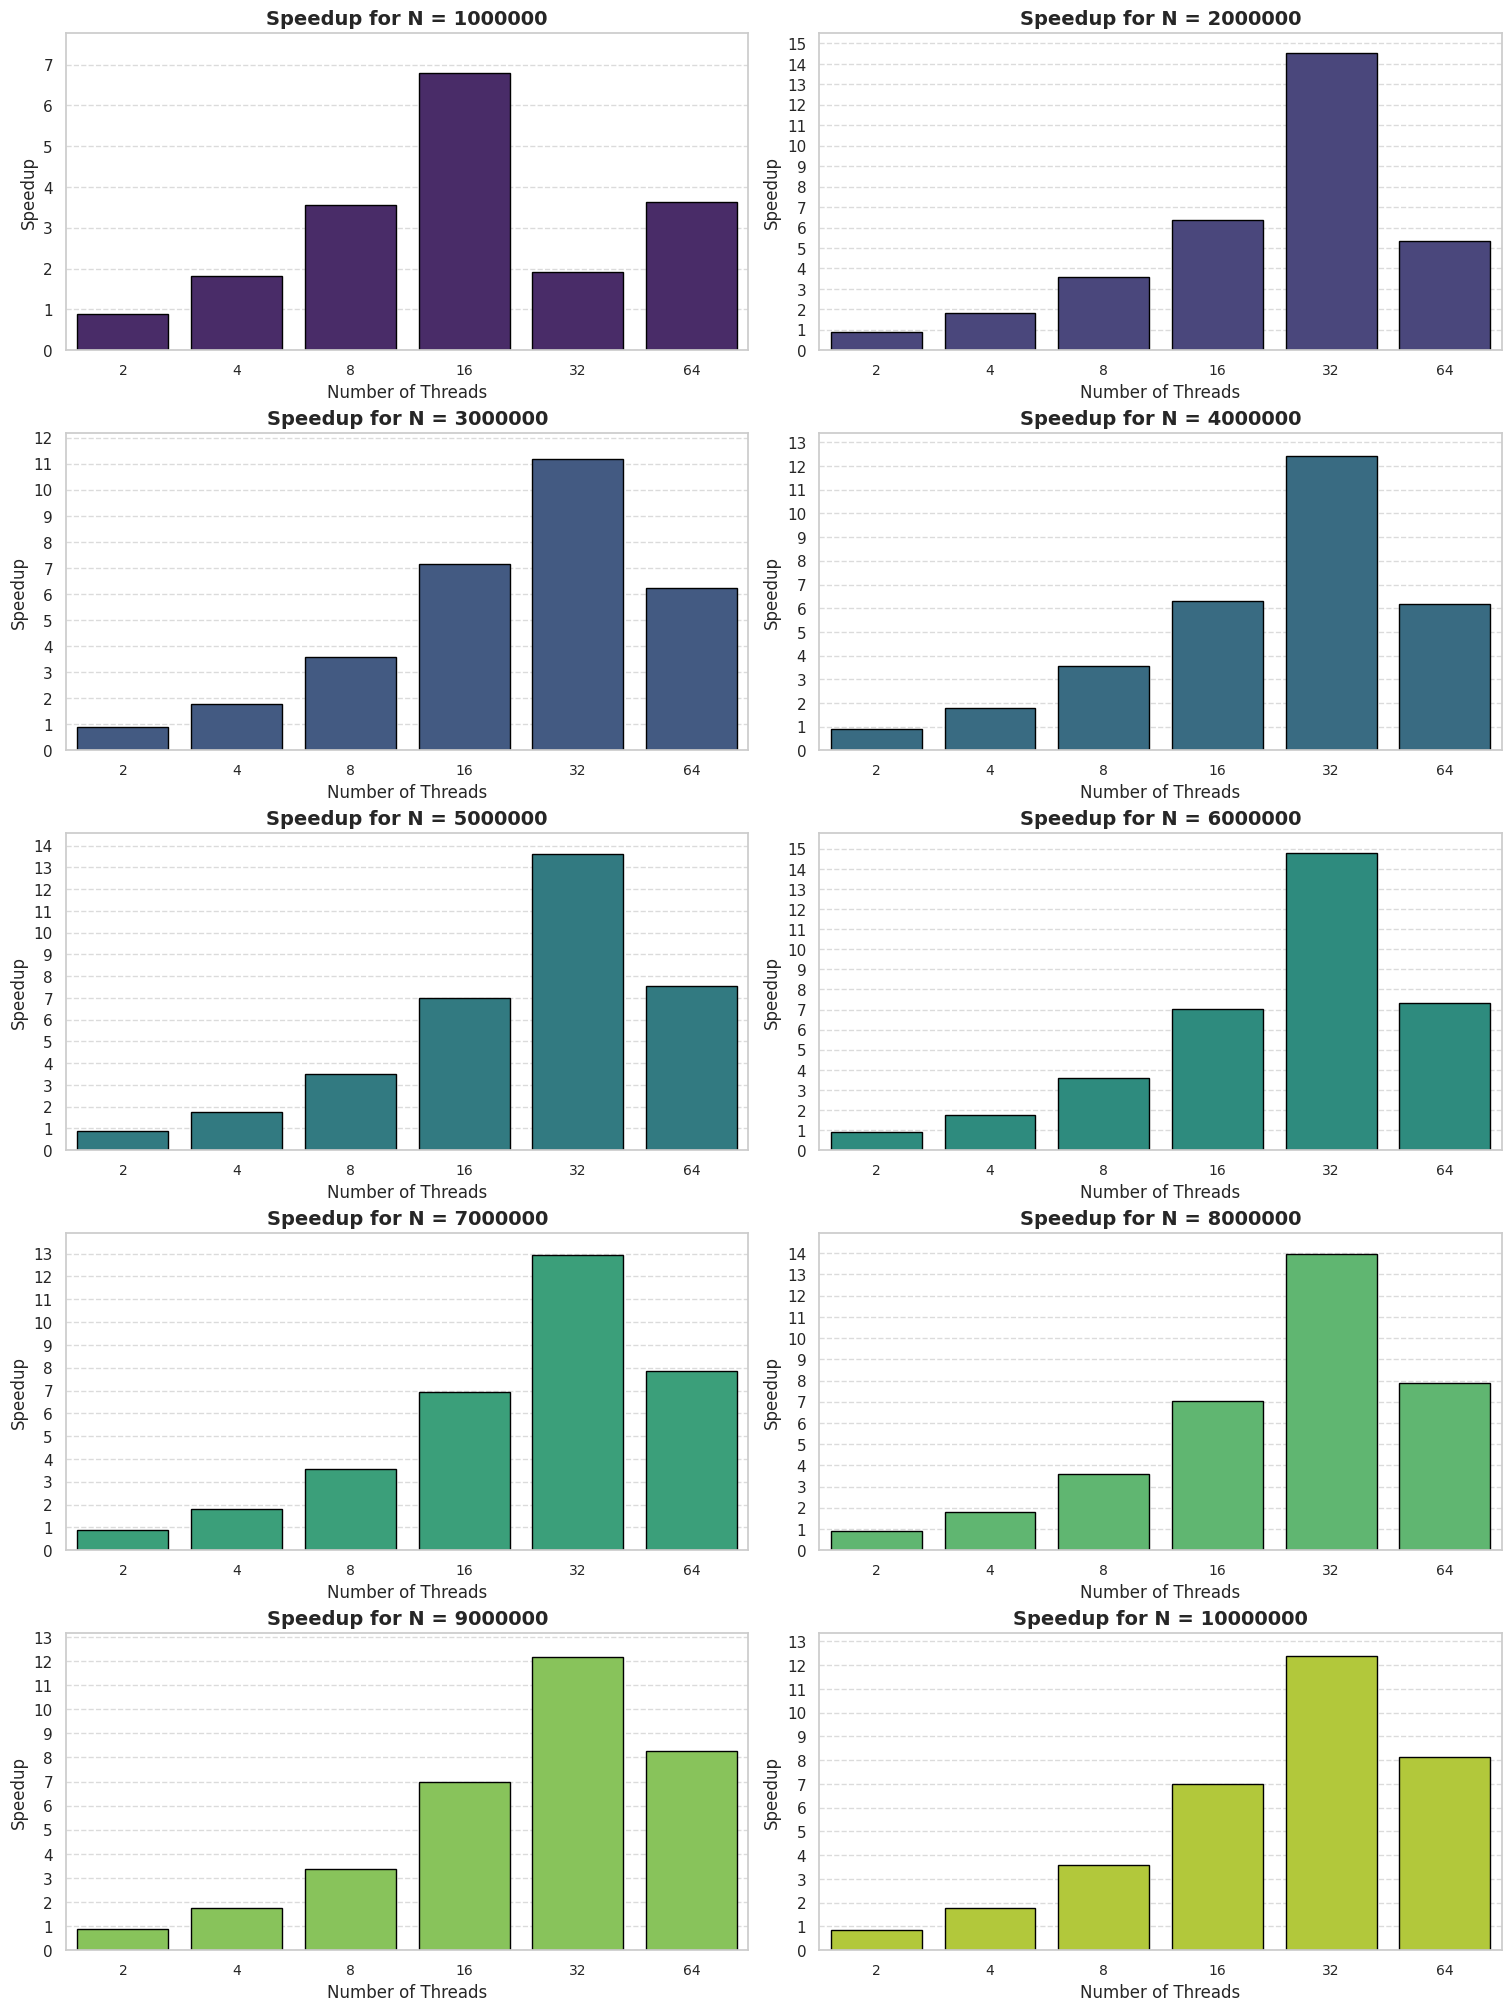
\includegraphics[width=0.95\textwidth]{images/omp_speedup_vs_t.png} % Adjust the width as needed
    \caption{Speedups for different N values.}
    \label{fig:parallel_vs-t}
\end{figure}
    
\begin{figure}[H]
    \centering
    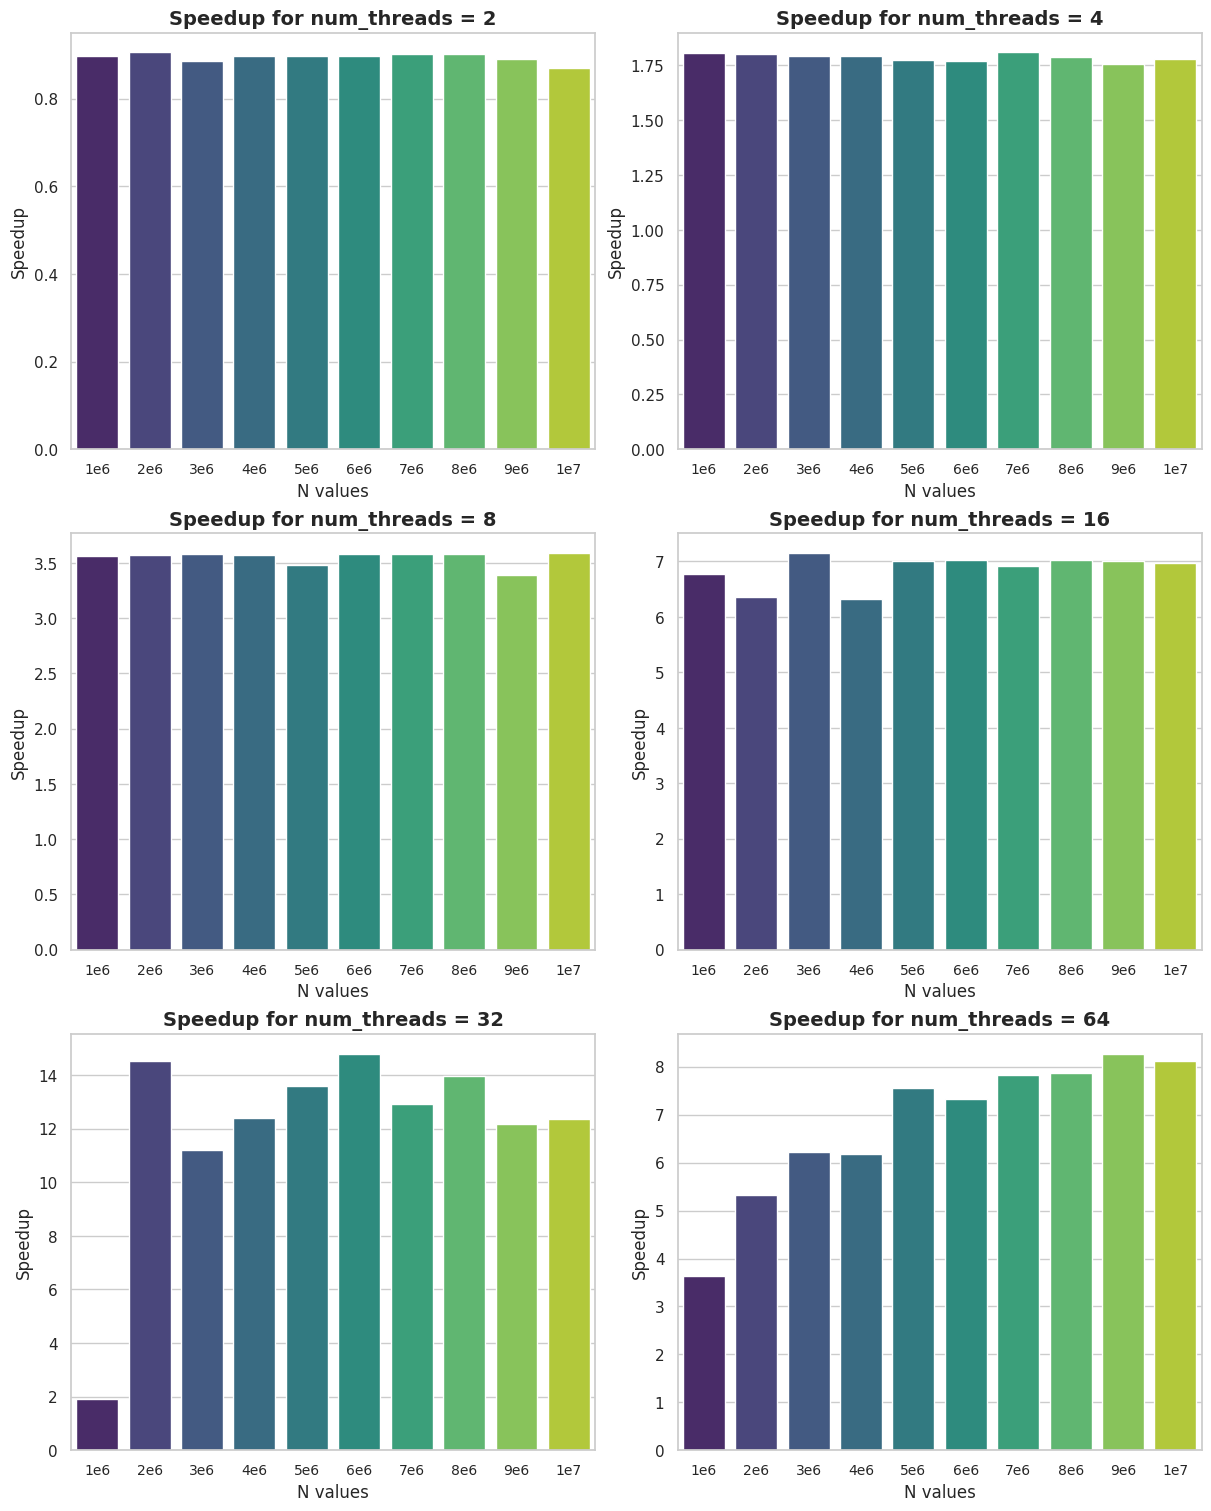
\includegraphics[width=1\textwidth]{images/omp_speedup_vs_N.png} % Adjust the width as needed
    \caption{Speedups for different num\_threads values.}
    \label{fig:parallel_vs-t}
\end{figure}
    
\begin{figure}[H]
    \centering
    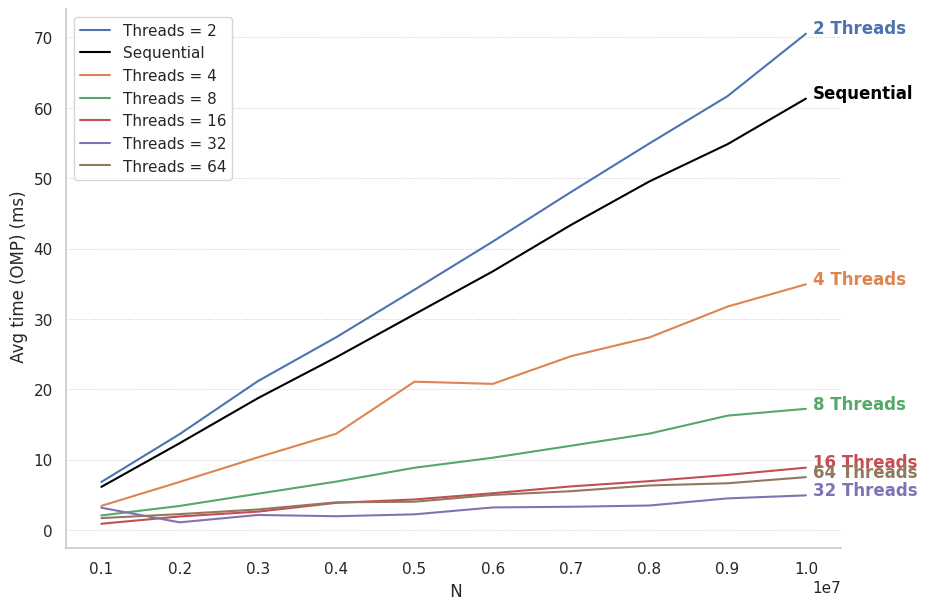
\includegraphics[width=1\textwidth]{images/openmp_time_vs_N.png} % Adjust the width as needed
    \caption{Time vs N plot for different values of num\_th}
    \label{fig:parallel_vs-t}
\end{figure}

\begin{tcolorbox}
\section*{4 Observations}
\end{tcolorbox}


\\

\begin{enumerate}
    \item \textit{\textbf{In Figure 3, for $num\_threads = 2$ we can see speeddowns across the board (around 0.9). }}: \\ This can be explained by the fact that the time complexity of the serial code is $O(n)$ and that for parallel with t = 2 is : $$O(\frac{2n}{2} + 2)) + parallelization\ overheads $$
    $$ = O(n) + parallelization\ overheads$$

    These parallelization overheads are the reason for slowdown. Therefore with our methodology, \textbf{\textit{we need at least two cores to almost approximately match the performance of the serial code.}}

    \item \textit{\textbf{In Figure 2, There is a slowdown for num\_threads = 64 for every value of N (almost half of peak)}}: \\

    \begin{figure}[H]
        \centering
        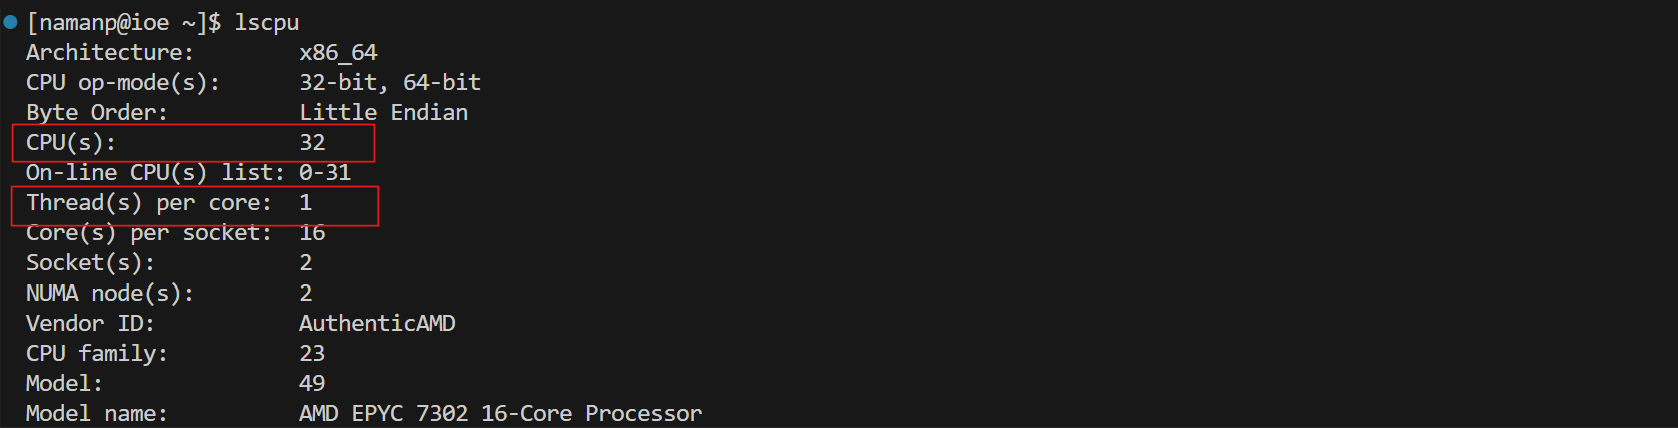
\includegraphics[width=0.9\textwidth]{images/LSCPU.png} % Adjust the width as needed
        % \caption{Speedups for different num\_threads values.}
        \label{fig:parallel_vs-t}
    \end{figure}
    This is because the CPU provided to us for our profiling purposes has 32 cores and can execute 1 thread per core. $$32*1 = 32 \text{ concurrent threads}$$ Assigning 64 threads means multiple threads must share each core, leading to \textbf{\textit{context switching overhead}}. and hence a slowdown.

    \item \textbf{\textit{In Figure 2, for N = 1000000, we see a slowdown for num\_threads = 32}}: \\
    One explanation to this is because the \underline{parallelization overhead} overtakes the time complexity for small N.

    \item \textbf{\textit{From Figure 3, except for very large t values (32 and 64), we see that the speedup is almost in a constant range.}}

    \item \textbf{\textit{The average speed up values double for every num\_thread doubling (till num\_threads = 32 because of obs 2 )}}: 

    We can see from the both Figures 2 and 3, that the speedup doubled for every doubling in threads. This is consistent with our time complexity analysis as $t << n$ :

    \[
    T(n,t) = O\left(\frac{2n}{t} + t\right)
    \]

    \[
    T(n,t) \approx O\left(\frac{2n}{t}\right) \text{ as } t << n
    \]

    \[
    T(n,2t) \approx  O\left(\frac{2n}{2t}\right) =  O\left(\frac{n}{t}\right) = \frac{1}{2}O\left(\frac{2n}{t}\right) = \frac{1}{2} T(n,t)
    \]

    \[
    \frac{1}{T(n,2t)} = 2 \frac{1}{T(n,t)}
    \]

    \[
    \frac{T(n,1)}{T(n,2t)} = 2 \frac{T(n,1)}{T(n,t)}
    \]
    
    \begin{center}
    \begin{tcolorbox}[width=0.22\textwidth]
     $S(n, 2t) = 2 {S(n,t)}$ 
    \end{tcolorbox}
    \end{center}

\\

\hrule
\end{enumerate}

\end{question}


\begin{question}{Q2 \underline{MPI Finding an element in a large array(7.5 points)}

Refer to the MPI class lecture slides that has a MPI program involving two processes that tries to find a particular element in an array distributed across the two processes. Now write a MPI program that works with any number of processes.

For this program, generate a random integer array of size 1000000 (i.e., 1 million) with random integer elements between 1 to 5000000 (5 million). You can either generate this array in process 0 and distribute it equally across all the processes or generate this array to a file and make the processes read from different portions of the file (e.g., using fseek). Now an integer element is given as input to the program and the processes start searching for this element in their local sub arrays. As soon as a process finds the element, it informs the other processes and all processes will stop searching. Process 0 should print the global index of the overall array in which the element was found.

Execute the program with different number of processes including 1 (sequential), 8, 16, 32 and 64. For each number of processes, execute with 20 different random input numbers for searching and in each case, measure the time taken for the search. Report the average time (across the 20 instances) taken for each number of processes. Plot the execution times and speedups for different number of processes. Ensure that you execute different processes on different cores.
Prepare a report with the methodology, execution times, and speedup graphs.}


\begin{tcolorbox}
    \section* {1 Methodology}
\end{tcolorbox}

\begin{tcolorbox}
    \section* {2 Experiments}
\end{tcolorbox}

\begin{tcolorbox}
    \section* {3 Results }
\end{tcolorbox}

\begin{tcolorbox}
    \section* {4 Observations}
\end{tcolorbox}




\end{question}


\begin{question}{APPENDIX 1: Parallel openmp prefix sum results}
\lstinputlisting{openmp/results.txt}
\end{question}

\begin{question}{APPENDIX 2: Parallel MPI find\_max results}
\lstinputlisting{mpi/results.txt}
\end{question}

\end{document}



